%% This is an example first chapter.  You should put chapter/appendix that you
%% write into a separate file, and add a line \include{yourfilename} to
%% main.tex, where `yourfilename.tex' is the name of the chapter/appendix file.
%% You can process specific files by typing their names in at the 
%% \files=
%% prompt when you run the file main.tex through LaTeX.
\chapter{Examples and Results}
This chapter will describe the results of my work using an excerpt of of W. A. Mozart's \textit{Eine Kleine Nachtmusik, K.525- I.Allegro} (referred to by just ``K.525'' from here onwards) as an example. It will also use an excerpt of W. A. Mozart's \textit{String Quartet No.7 in E-flat major, K.160- I.Allegro} (referred to by just ``K.160'' from here onwards) as an example where K.525 doesn't fit the specifications. This chapter will also look at timing metrics of the system.

\section{Eine Kleine Nachtmusik, K.525- I.Allegro, W. A. Mozart}		
This section will go through an example of how the entire \texttt{OMRMIDICorrector} system works on W. A. Mozart's \textit{Eine Kleine Nachtmusik, K.525- I.Allegro}.

\begin{figure}[H]
\centering
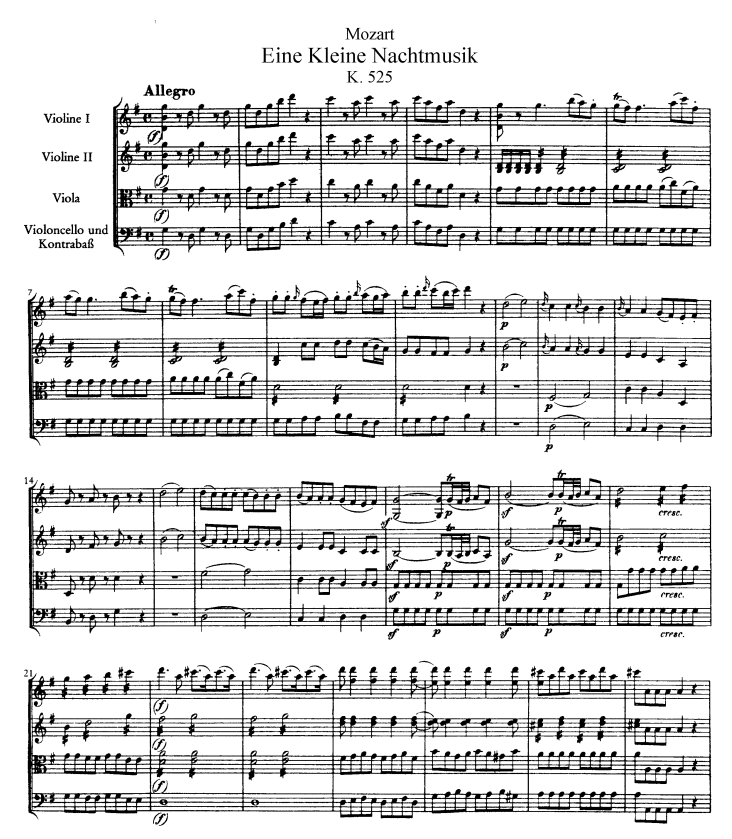
\includegraphics[width =.9\textwidth]{k525originalomrscan}
\caption{The first page of the scanned copy of the score found on IMSLP.}
\end{figure}

\subsection{Musical Properties of K.525}
I chose K.525 as the example piece for its many music properties that make it a difficult but interesting piece to align.

\subsubsection{Bass and Cello Doubling}
In the original scanned score, there are only four parts because the bass part doubles the cello part one octave lower. However, in the MIDI encoding, there are five separate voices. Thus, in the preprocessing step of the \texttt{OMRMiDICorrector}, it would be ideal for the system to recognize this. Otherwise, in instances where the \texttt{OMRMIDICorrector} could not pair up the parts between the input OMR stream and the input MIDI stream, there would be an error thrown, and alignment and correction would not happen. 

\subsubsection{Tremolos}
Starting in measure 5 in the original scanned score, the second violin has tremolo notes, instead of repeated \nth{16} notes written out. The OMR parser in SmartScore is not robust enough to recognize the slashes across the stem of the note as tremolo markings and instead interprets it as a single note. The MIDI protocol has no way of indicating tremolos, so the second violin's notes in measure 5 are encoded as regular \nth{16} notes. The \texttt{Aligner} is robust enough to align tremolo measures with non-tremolo measures even though there is a huge discrepancy in the number of notes present in the measure.

\subsection{Preparing the Raw Input}
The basic raw input of the system is an OMR score and a MIDI file. A scanned copy of the score was found in IMSLP \cite{k525}, the source for much free public domain sheet music. The MIDI file was sourced from the Yale MIDI Archive. 

I used SmartScore's built-in OMR tool to convert the scanned score of K.525 into an ENF file. Then I exported the post-OMR file as a musicXML file.

Similarly for the K.525 MIDI file, I used SmartScore to parse the original file and exported it as a musicXML file. 

The last step of preparing the raw input is to parse the musicXML files with the \texttt{music21} library so that they are \texttt{Stream} objects. This can be done by passing in the musicXML filepaths to the \texttt{parse} method in the \texttt{converter} class. We will call these two parsed streams \texttt{k525midiStream} and \texttt{k525omrStream}. 
\begin{minted}{python}
from music21 import *
k525MidiFilepath = "pathto/k525mvmt1/miditoxml.xml"
k525OmrFilepath= "pathto/k525mvmt1/omrtoxml.xml"
k525midistream = converter.parse(k525MidiFilepath)
k525omrstream = converter.parse(k525OmrFilepath)
\end{minted}
\subsection{Running \texttt{OMRMIDICorrector} on K.525}
After the raw input has been massaged into \texttt{Stream} objects, the aligning process is simple. We create an instance of an \texttt{OMRMIDICorrector} object with the two streams as parameters. For the purposes of this example, we will use the default hasher that is built into the \texttt{OMRMIDICorrector} class. We will set the \texttt{debugShow} to \texttt{True} so that we can visualize the alignment between pairwise streams. Finally, we will call \texttt{processRunner} which will hash and align the parts in the stream. For now, we will manually create the \texttt{Fixer} objects for stream fixing. The aligner is able to correctly identify that the repeated \nth{16} notes 

\begin{minted}{python}
from music21 import *
OMC = alpha.analysis.omrMidiCorrector
k525omc = OMC.OMRMIDICorrector(k525midistream, k525omrstream)
k525omc.debugShow = True
k525omc.processRunner()
\end{minted}

The outputs of the \texttt{showChanges} function are all in Appendix \ref{appb}

\subsubsection{A Closer Look at Specifics of \texttt{processrunner}}
A lot of magic happens within \texttt{processRunner}, all of which was described at a high level in sections \ref{processrunner1} - \ref{processrunner2}. Here are some salient details of the process in the context of K.525 that I think deserve notice:
\begin{itemize}
\item Bass Doubles Cello Part - The OMR score has only four parts, whereas the MIDI score has 5. The \texttt{checkBassDoublesCello} method in \texttt{OMRMIDICorrector} is able to correctly identify this and thus does not reject the input on the basis of having a mismatching number of parts in the stream. 
\item Rhythmic Fault Tolerance: Beginning Rests - The first measure in the OMR score is a scanning and parsing error. The \texttt{Aligner} is robust enough to identify the beginning rest as a insertion error. 
\item Rhythmic Fault Tolerance: Propagating Rhythmic Shifts - By measure 5 in the Violin 2 part, we see that the OMR score has introduced a \nth{16} note shift in the rhythm which continues for a few measures. 
\item Notation Fault Tolerance: Tremolos - By measure 5 of the Violin 2 part and by measure 10 of the Viola part, the repeated \nth{16} notes get notated with tremolo slashes in the original OMR score. Of course, the MIDI protocol doesn't have a way of representing tremolo, so the notes are written out in long form. The corrector is able to match the written out repeated notes in the MIDI to the (incorrectly) scanned corresponding notes in the OMR. 
\end{itemize}

\subsection{Example 1: Similarity Metrics in K.525}
Recall that the \texttt{similarityScore} is the ratio of \texttt{NoChange} operations to the total number of operations in the \texttt{changes} list. For each pair of streams in K.525, the \texttt{similarityScore} and \texttt{changesCount} are listed below:
\begin{table}[H]
\centering
\begin{tabular}{lll}
           & \texttt{similarityScore} & \texttt{changesCount}                                                  \\
Violin 1   & 0.51                       & \{NoChange: 83, Ins: 30, Del: 10, Sub: 39\} \\
Violin 2   & 0.30                       & \{NoChange: 74, Ins: 125, Del: 9, Sub: 38\} \\
Viola      & 0.72                       & \{NoChange: 97, Ins: 21, Del: 9, Sub: 8\}   \\
Cello/Bass & 0.87                       & \{NoChange: 107, Del: 11, Sub: 5\}               
\end{tabular}
\caption{\texttt{similarityScore} and \texttt{changesCount} for every pair of aligned streams}
\end{table}

A visual examination of the pairs of streams suggests that these numbers and counts look correct. The Cello/Bass parts have the fewest colorations to their notes and no insertion changes at all. The least similar pair of parts is the Violin 2, which has multiple cases of the tremolo problem described above as well as propagating rhythmic shifts.

\section{String Quartet No.7 in E-flat major, K.160- I.Allegro, W. A. Mozart}
The previous section showed the alignment between parts in \textit{Eine Kleine Nachtmusik}. In this section will use another piece by Mozart to demonstrate how the \texttt{EnharmonicFixer} works on correcting an excerpt of the Violin 1 part of K.160. This OMR score was also sourced from IMSLP \cite{k160}.

\subsection{Running \texttt{EnharmonicFixer} on K.160, Violin 1}
After prepping the raw input files of K.160 in the same way as detailed above and running that through an \texttt{OMRMIDICorrector} instance, we will create an \texttt{EnharmonicFixer} instance using just the Violin 1 OMR stream and MIDI stream and the associated \texttt{changes} list.

\begin{minted}{python}
from music21 import *
k160MidiFilepath = "pathto/k160mvmt1/miditoxml.xml"
k160OmrFilepath = "pathto/k160mvmt1/omrtoxml.xml"
         
k160midiStream = converter.parse(k160MidiFilepath)
k160omrStream = converter.parse(k160OmrFilepath)
k160omc = OMRMIDICorrector(k160midiStream, k160omrStream)
k160omc.processRunner()
        
V1Changes = k160omc.changes[0]
V1Midi = k160omc.midiParts[0]
V1Omr = k160omc.omrParts[0]
k160EF = fixer.EnharmonicFixer(V1Changes, V1Midi, V1Omr)
k160EF.fix()

k160omcViolin1OmrStream.show()
\end{minted}

In Appendix\ref{appb}, the first two figures below show the alignment visualization of the Violin 1 part. The last figure shows the corrected OMR score after it has been changed by the \texttt{EnharmonicFixer}.

\subsection{Analysis of Correction}
Visual inspection of figures \ref{fig:k160postalignv1midi} and \ref{fig:k160postalignv1omr} suggests that the OMR failed to pick up the appropriate key signature of the movement and that is what lends to large number of changes in the first 10 or so measures. Inspection of figure \ref{fig:k160postfixv1} shows that many of the pitch errors have been corrected using the \texttt{EnharmonicFixer}. Of course, the most ideal scenario would be to recreate the key signature, but having the correct pitch is a good start. 

\section{Results: Timing Tests} \label{timing}
This section will evaluate the runtime on each of the three major modules of the system the \texttt{Hasher}, \texttt{Aligner}, and\texttt{Fixer} as well as the entire system, \texttt{OMRMIDICorrector} which is a combination of some number of instances of the three major modules. It will also discuss how the system would scale to different sized inputs. 

For the following calculations, assume that the length of the input MIDI stream and the OMR stream are about the same, $n$, and that the number of parts in each of the streams is $p$. 

\subsection{Runtime Analysis: \texttt{Hasher}}
Setup of the \texttt{Hasher} object is in $O(n)$ time. Building the list \texttt{finalEltsToBeHashed} requires scanning the input stream in full. Recall that the \texttt{tupleList} is a list of the stream element properties that will be hashed; call its length $t$. The runtime of the \texttt{hashStream} method is then $O(k \cdot n)$. 

Thus, a single use of the \texttt{Hasher} is in $O(n) + O(k \cdot n) = O(n)$ time for small $k$. This is a reasonable assumption because the number of notes in a stream is likely to be far greater than the number of possible qualities of stream elements that can be hashed. 

\subsection{Runtime Analysis: \texttt{Aligner}}
Setup of a \texttt{StreamAligner} object takes $O(n \cdot n) = O(n^2)$ time, dominated by the \texttt{populateDistanceMatrix} function. Traceback in the \texttt{calculateChangesList} method takes $O(n+ n) = O(n)$ time. The length of the \texttt{changes} list is then also $O(n)$. The runtime of \texttt{showChanges} is proportional to the length of the \texttt{changes} list, calculated above to be $O(n)$

A single use of a \texttt{StreamAligner} object is in $O(n^2) + O(n) +O(n) = O(n^2)$ time. 

\subsection{Runtime Analysis: \texttt{Fixer}}
The \texttt{OMRMIDIFixer} and the \texttt{EnharmonicFixer} both require negligible setup. The \texttt{fix} function's runtime is proportional to the length of the \texttt{changes} list input, shown above to be $O(n)$. 

A single use of a \texttt{Fixer} object is in $O(n)$ time. 

\subsection{Runtime Analysis: \texttt{OMRMIDICorrector}}
For a single instance of an \texttt{OMRMIDICorrector} with OMR and MIDI streams of length $n$ and $p$ parts, there are $2 \cdot p$ texttt{Hasher} objects, $p$ \texttt{Aligner} objects, and $p$ \texttt{Fixer} objects created. In total this comes out to a time of:
$$2 \cdot p \cdot O(n) + p \cdot O(n^2) + p \cdot O(n)$$
$$ = p \cdot O(n^2) + 3 \cdot O(n)$$ For small $p$, this collapses to $O(n^2)$. 
 
\subsection{Empirical Results}
Using the the first movement of K.160, I timed some results using the \texttt{\% timeit} functionality of iPython. First I tested the major modules on a single stream, the Violin 1 part of K.160. Then I tested the OMR/MIDI Correction system on all of the K.160.

\subsection{\texttt{\%timeit}: Hasher}
After setting up a \texttt{Hasher}, \texttt{\% timeit}  reported an average time of 621 ms per call to hash the MIDI stream and average time of 617 ms per call to hash the OMR stream. The length of the hashed MIDI stream was 662 and and the length of the hashed OMR stream was 669. 

\subsection{\texttt{\%timeit}: Aligner}
After setting up a \texttt{StreamAligner} object using the hashed MIDI stream and the hashed OMR stream, I ran \texttt{\% timeit} on the \texttt{align} function and got an average of 2.39 s per call. Since the \texttt{align} function itself hashes input streams if not already hashed, I passed in the hashed streams. This produced more accurate measurement of the time for the alignment process, separate from the hashing process.

\subsection{\texttt{\%timeit}: Fixer}
I set up a \texttt{EnharmonicFixer} object using the \texttt{changes} list from the aligning step and the original K.160 Violin 1 OMR and MIDI streams. Running \texttt{\% timeit} on the \texttt{fix} function returned an average of 12.7 ms per call. 

\subsection{\texttt{\%timeit}: OMR/MIDI Corrector}
After testing the timing of each of the major modules, I tested the timing of the OMR/MIDI Correction system on the entire first movement of K.160. The average time to hash, align, and fix the four instrumental parts in K.160 was 12.94 s. 

An entire run of the OMR/MIDI Corrector system on K.160 require 8 calls to the \texttt{Hasher}, 4 calls to the \texttt{Aligner}, and 4 calls to the \texttt{Fixer}. Using the empirical numbers from above, this gives an estimate of 14.56 seconds, which is in the range of the 12.94 seconds that \texttt{\%timeit} gives us. The speedup in the empirical time versus the calculated time likely comes from the fact that there is considerable setup that was reused in calling the \texttt{OMRMIDICorrector} once instead of its constituent modules. 

\subsection{Scalability}
If a single movement of a four-part Mozart quartet takes on the order of tens of seconds to hash, align, and fix, then most multi-movement pieces for chamber ensembles should take on the order of minutes to hash, align, and fix. Larger orchestral works might take on the order of tens of minutes to hash, align, and fix. Especially for the first system of its type, these preliminary timings of the \texttt{OMRMIDICorrector} have good implications. 

The bottleneck of the system lies in the \texttt{Aligner}. The method implemented in my system is a basic string alignment algorithm, and there is considerable room for speedup using techniques such as The Four Russian Algorithm \cite{seqalign}. 

\subsection{Implications of Free Music}
The lasting and tangible results of this research will hopefully be in helping providing more free and high-quality musical scores to the public. With ISMLP alone having over 350,000 scores that are freely available, there is a lot of potential for my work to liberate otherwise sub-quality scanned musical scores and turn them into digital scores that can be conveniently analyzed, replicated, and distributed. It's my hope that this work will be able to facilitate musical research, provide individuals and groups with easy access to practice material, and help bring more music to all of our lives.
